\section{Objektliste}
\thispagestyle{fancy}

Grunna arbeidet rundt konstruksjonen av \gls{PID} valge vi også å lage ei liste over alle komponenante i anlegget som var tilkopla og styrt av styresystemet.
Objektlista inneheld utstyrsbeskrivelse, plassering og tag. 

I arbeidet rundt innhenting av informasjon til dei ulike objekta vi skulle styre har vi også laga til eit datablad-database,
som inneheld relevant informasjon til kvar enkelt komponent i styresystemet.\newline
Desse datablada er tilgjengeleg i appendix (Appendix xXx)

I PLS programmet har vi brukt tags når vi definerer blokker og navngir komponentar. \newline
Denne lista vil gi moglegheit for å knytte korrekt tag opp mot riktig komponent.



\newpage

\begin{tikzpicture}[remember picture, overlay]
    % Include the PDF page rotated, positioned at the center of the page
    \node[inner sep=0pt] at (current page.center) {
        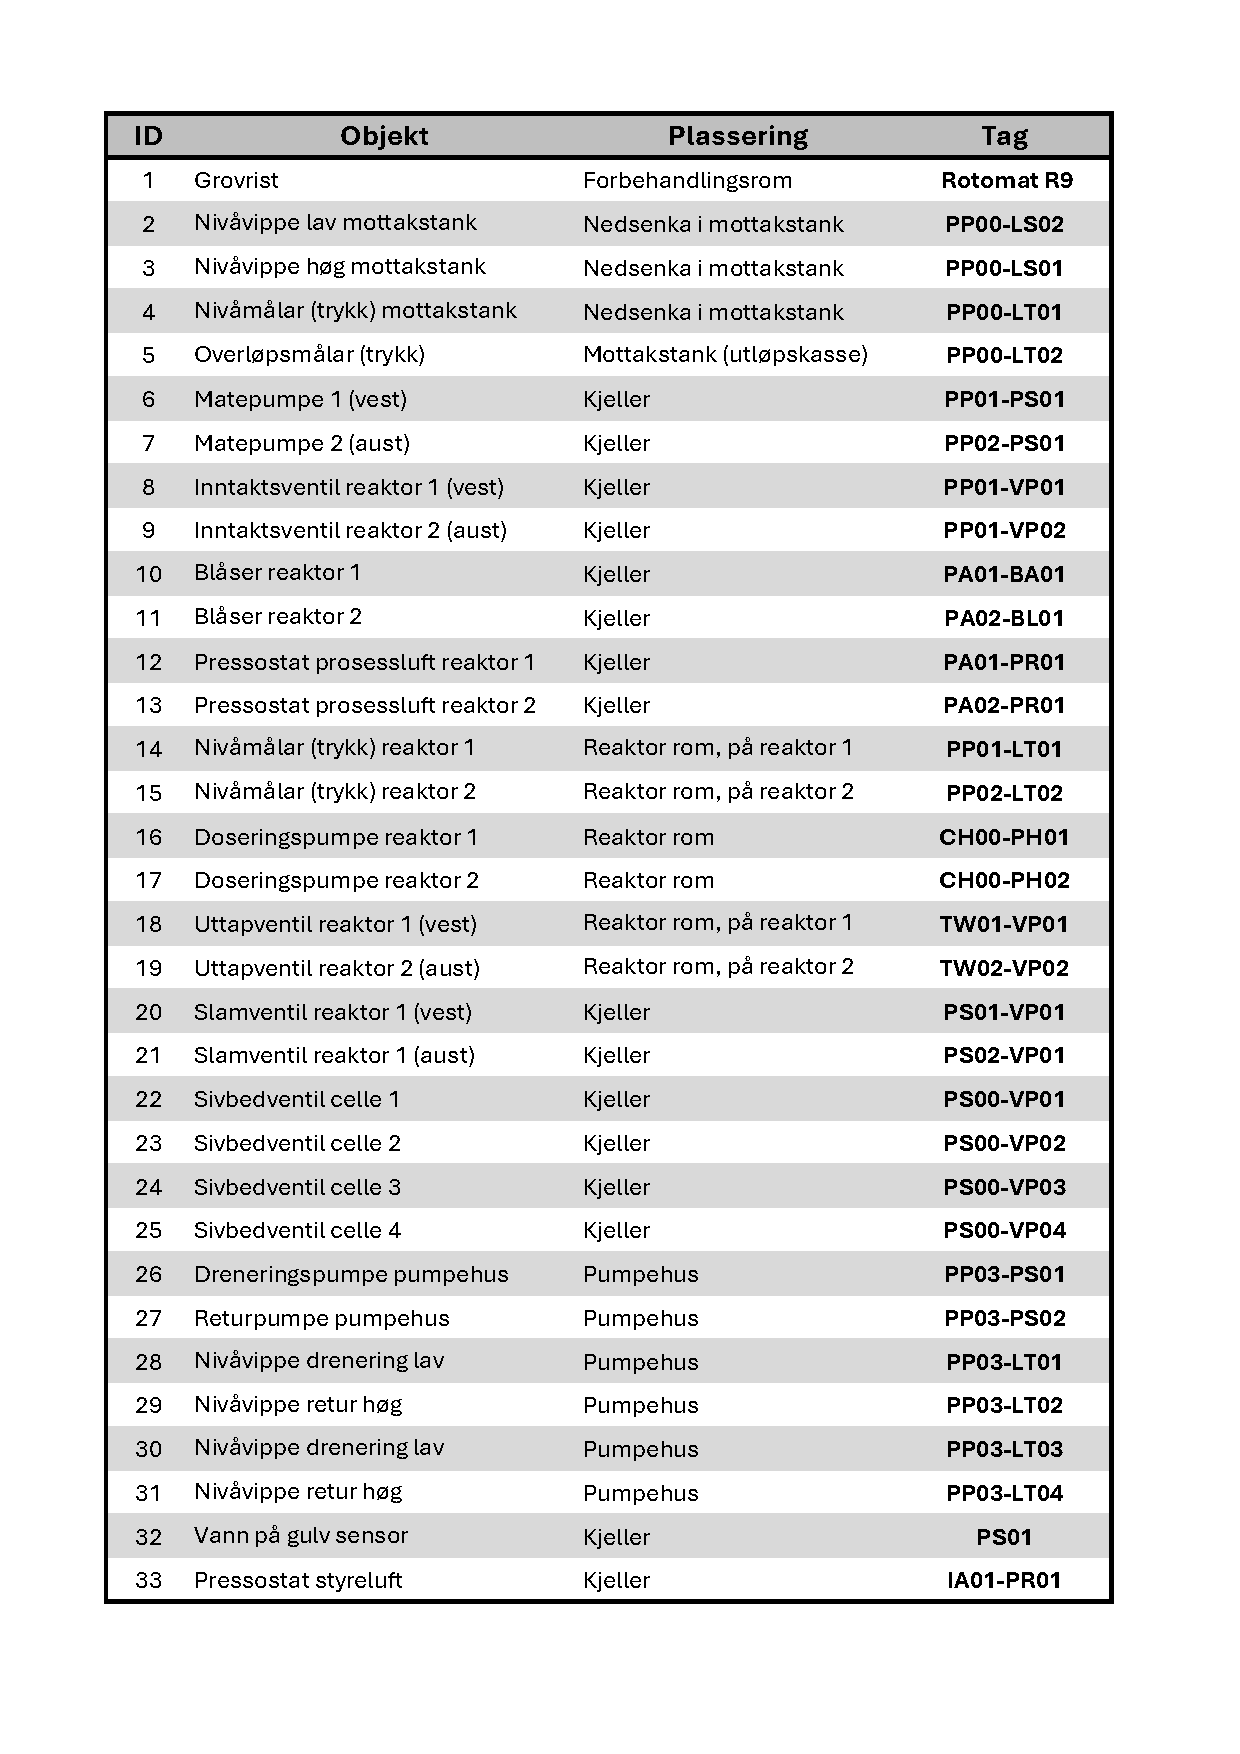
\includegraphics[page=1, scale=1, keepaspectratio]{Bilder/NyKomponentliste.pdf}
    };

    % Place the caption at the bottom of the page
    \node[anchor=south, yshift=10mm] at (current page.south) { % Adjust yshift to position the caption
        \begin{minipage}{\textwidth}
            \centering
            \captionof{figure}{Objektliste}
            \label{fig:SCD}
        \end{minipage}
    };
\end{tikzpicture}
